% Created 2018-06-26 Tue 13:06
% Intended LaTeX compiler: pdflatex
\documentclass[captions=tableheading]{beamer}
\usepackage[utf8]{inputenc}
\usepackage[T1]{fontenc}
\usepackage{graphicx}
\usepackage{grffile}
\usepackage{longtable}
\usepackage{wrapfig}
\usepackage{rotating}
\usepackage[normalem]{ulem}
\usepackage{amsmath}
\usepackage{textcomp}
\usepackage{amssymb}
\usepackage{capt-of}
\usepackage{hyperref}
\usepackage{minted}
\usepackage{charter}
\usetheme{Frankfurt}
\useinnertheme{circles}
\usecolortheme{seagull}
\definecolor{UBCblue}{rgb}{0.04706, 0.13725, 0.26667} % UBC Blue (primary)
\definecolor{UBCgrey}{rgb}{0.3686, 0.5255, 0.6235} % UBC Grey (secondary)
\definecolor{UBCblack}{rgb}{0.011, 0.011, 0.011} % UBC Blue (primary)
\usecolortheme[named=UBCblue]{structure}
\setbeamercolor{palette secondary}{bg=UBCblue,fg=white}
\setbeamercolor{palette tertiary}{bg=UBCblue,fg=white}
\setbeamercolor{palette quaternary}{bg=UBCblack,fg=white}
\usepackage[margin=0.85in]{geometry}
\usemintedstyle{default}
\usetheme{default}
\author{Rchid Anas}
\date{}
\title{Informatiser le service Ressources Humaines chez la Faculté des Lettres et Science Humaines}
\hypersetup{
 pdfauthor={Rchid Anas},
 pdftitle={Informatiser le service Ressources Humaines chez la Faculté des Lettres et Science Humaines},
 pdfkeywords={},
 pdfsubject={},
 pdfcreator={Emacs 25.2.2 (Org mode 9.1.5)},
 pdflang={English}}
\begin{document}

\maketitle
\tableofcontents
\clearpage

\section{Introduction}
\label{sec:org98b21ab}
\begin{frame}[label={sec:orgd43bd1d}]{Introduction}
\begin{quote}
Ce projet est le résultat d'un stage que j'avais passé chez la \emph{Faculté des Lettres et Science Humaines}, El Jadida sous le thème \emph{Informatiser le service Ressources Humaines}. Sous l'encadrement de Mr. A. Madani, et la supervision du chef de service; Mr. Driss Dibaji.\\
\end{quote}
\end{frame}

\section{Cahier des Charges}
\label{sec:org63e5b2e}
\begin{frame}[label={sec:org421f763}]{Cahier des Charges}
Un service qui est responsable de la gestion des employés et fonctionnaires, leurs diplômes et grades\ldots{}\\
\pause

\begin{quote}
\begin{itemize}
\item Implémenter un système de gestion des employés/fonctionnaires \pause
\item Gérer les diplômes et les grades \pause
\item Suivi des grades \pause
\item Suivi d'absence \pause
\item Suivi de rémunération du travail les fériés \pause
\item Générer des attestations de travail \pause
\item Générer des autorisations de congé \pause
\item Générer des fiches de notation annuelle
\end{itemize}
\end{quote}
\end{frame}

\section{Conception}
\label{sec:orgab0bc2d}
\begin{frame}[fragile,label={sec:org3a43591}]{Conception}
 \begin{block}{Stockage des données en XML}
\pause
Les données sont stockées dans un fichier \texttt{XML}; \pause \alert{puisqu'il est lisible à la fois par la machine et l'humain}.\\

\pause\\

\begin{quote}
\begin{itemize}
\item Le root-tag est \texttt{<Employee>} et qui contient \alert{\texttt{0} ou plusieurs} tags de type \texttt{<employee>} qui représente des employées. \\
\end{itemize}
\pause
\begin{itemize}
\item Chaque tag \texttt{<employee>} contient \alert{un seul} tag \texttt{<personal>} et \alert{un seul} tag \texttt{<administrative>} qui peut contient \alert{\texttt{0} ou plusieurs} tags \texttt{<uplift>}. \\
\end{itemize}
\pause
\begin{itemize}
\item Le tag \texttt{<employee>} peut aussi avoir \alert{\texttt{0} ou plusieurs} tags de type \texttt{<diploma>}, \texttt{<medicalcertif>} et \texttt{<repayment>}.\\
\end{itemize}
\end{quote}
\end{block}
\end{frame}

\begin{frame}[fragile,label={sec:org40a3538}]{Les Paquets et leurs Classes}
 \clearpage

Le code source de l'application est divisé en 4 paquets pricipales: \pause

\begin{description}
\item[{\texttt{model}}] contient les différentes classe pour mobilisé les donnée en objet \pause
\item[{\texttt{app}}] contient les différentes énumération utilisées dans l'application. \pause Ce paquet contient aussi  \texttt{app.utils}, qui contient des utilitaires utiles pour le développement, notamment la gestion du \alert{fichier XML} \pause
\item[{\texttt{wins}}] contient des interfaces graphiques, y compris celles qui sont responsables des opérations CRUD normales qui existent dans \texttt{wins.crud} \pause
\item[{\texttt{views}}] contient des pages générées pour l'impression.
\end{description}
\end{frame}

\begin{frame}[fragile,label={sec:orgc6680c5}]{Paquet \texttt{app}}
 Ce paquet contient que les énumérations \pause
\begin{center}
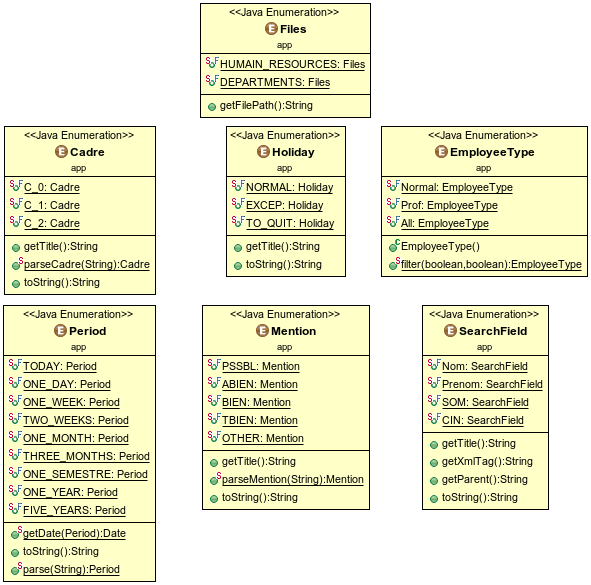
\includegraphics[width=7cm]{./diags/OverviewOnApp.png}
\end{center}
\end{frame}
\begin{frame}[fragile,label={sec:org65665a4}]{Paquet \texttt{app.utils}}
 \begin{center}
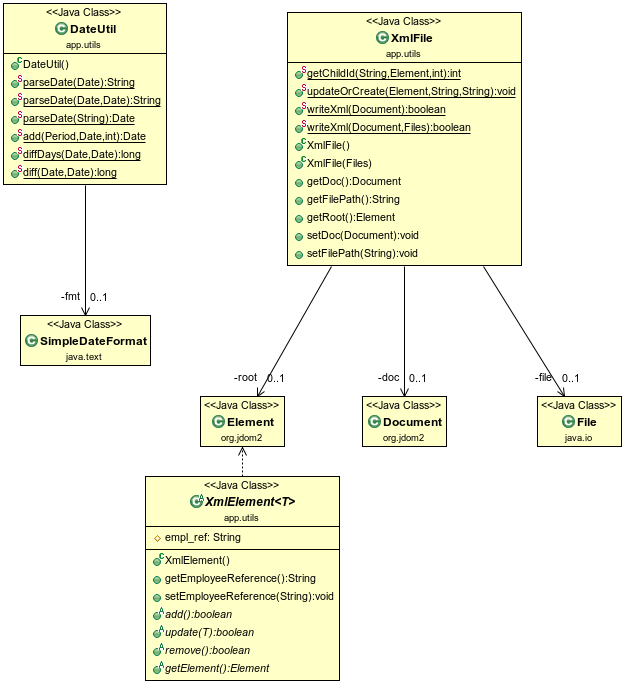
\includegraphics[width=7cm]{./diags/OverviewAppUtils1.png}
\end{center}
\end{frame}

\begin{frame}[fragile,label={sec:orgb473447}]{La classe \texttt{XmlFile}}
 \begin{quote}
\texttt{XmlFile}, la couche \emph{DAO} de l'application. Elle est responsable a tout interaction avec le fichier \texttt{XML}. Elle est basée sur un paquet \texttt{Java} appelée \texttt{JDOM}.
\end{quote}

\begin{block}{Les composant de JDOM}
\begin{description}
\item[{\texttt{Element}}] la représentation des tags XML en objet
\item[{\texttt{Document}}] la représentation du document XML en objet
\item[{\texttt{SAXBuilder}}] pour initialiser les instances \texttt{Document}
\item[{\texttt{XMLOutputter}}] pour l'écriture de \texttt{Document} et fichier réal
\end{description}
\end{block}
\end{frame}
\begin{frame}[fragile,label={sec:org8ad45b9}]{Les méthodes de la classe \texttt{XmlFile}}
 \begin{quote}
En peut sauvegarder les changements dans le fichier XML avec la méthode \texttt{static write Xml()}.
\end{quote}

\begin{block}{Définition de la méthode}
\begin{minted}[linenos,firstnumber=1]{java}
public static boolean writeXml(Document doc, Files f) {
    try {
        XMLOutputter out = new XMLOutputter( );
        out.setFormat(Format.getPrettyFormat( ));
        out.output(
            doc, new FileWriter(f.getFilePath( )));
        return true;
    } catch (IOException e) {
        return false;
    }
}
\end{minted}
\end{block}
\end{frame}
\begin{frame}[fragile,label={sec:org7bd06e2}]{Les méthodes de la classe \texttt{XmlFile}}
 \begin{quote}
Avec l'aide de \texttt{static updateOrCreate()} on peut faire une mise à jour a une valeur d'un tag dans le fichier \texttt{XML}.
\end{quote}
\begin{block}{Définition de la méthode}
\begin{minted}[linenos,firstnumber=1]{java}
public static void updateOrCreate(Element el,
                                  String node,
                                  String value) {
    if (el.getChild(node) == null) {
        el.addContent(
            new Element(node).addContent(value));
        writeXml(el.getDocument( ));
    } else {
        el.getChild(node).setText(value);
    }
}
\end{minted}
\end{block}
\end{frame}
\begin{frame}[fragile,label={sec:org7342f08}]{La classe \texttt{XmlElement}}
 \begin{minted}[linenos,firstnumber=1]{java}
public abstract class XmlElement<T> {
    public abstract boolean add();
    public abstract boolean update(T updated);
    public abstract boolean remove();
    public abstract Element getElement();

    /* référence du employé */
    protected String empl_ref;
    public String getEmployeeReference( ) {
        return empl_ref;
    }

    public void setEmployeeReference(String ref) {
        this.empl_ref = ref;
    }
}
\end{minted}
\end{frame}

\begin{frame}[fragile,label={sec:orgb62c5ad}]{La classe \texttt{DateUtil}}
 \begin{quote}
La classe \texttt{DateUtil} est utilisé pour la manipulation des dates, et la conversion des dates de/vers \texttt{String} avec l'aide du classe system \texttt{SimpleDateFormat}. Pour les dates, j'ai choisi un format standard, \texttt{YYYY-MM-DD}, pour touts les dates dans le projet.
\end{quote}

\begin{block}{Extrait de la classe}
\begin{minted}[linenos,firstnumber=1]{java}
public class DateUtil {
    private SimpleDateFormat fmt;

    public DateUtil() {
        fmt = new SimpleDateFormat("yyyy-MM-dd");
    }
}
\end{minted}
\end{block}
\end{frame}


\begin{frame}[fragile,label={sec:org200d449}]{Suite du Paquet \texttt{app.utils}}
 Ce paquet contient des classes important pour l'application. \pause
\begin{center}
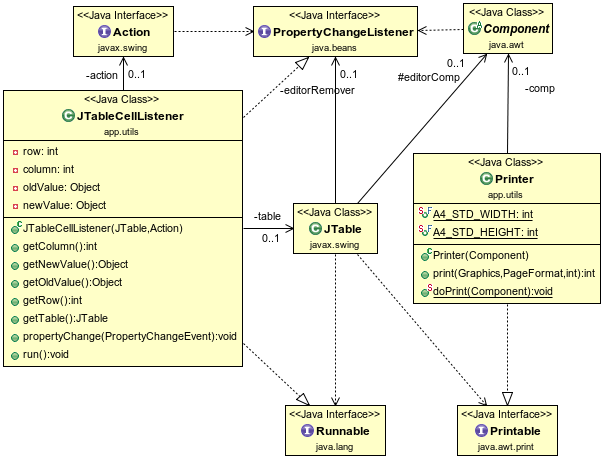
\includegraphics[width=9cm]{./diags/OverviewAppUtils0.png}
\end{center}
\end{frame}

\begin{frame}[fragile,label={sec:orga0eb7c7}]{La classe \texttt{Printer}}
 \begin{quote}
La classe \texttt{Printer} est responsable de l'impression d'un \texttt{Component} (la classe des composants graphiques) avec l'aide de la méthode \texttt{static doPrint()} qui prend un \texttt{Component} comme paramètre.
\end{quote}
\pause

\begin{block}{Example de l'appel}
\begin{minted}[]{java}
import app.utils.Printer;

Printer.doPrint(/* le composant graphique */);
\end{minted}
\pause
\end{block}
\begin{block}{Implémentation de l'interface \texttt{java.awt.Printable}}
\begin{quote}
Aussi, \texttt{Printer} a une implémentation de la méthode abstrait \texttt{print()} de l'interface \texttt{Printable}
\end{quote}
\end{block}
\end{frame}

\begin{frame}[fragile,label={sec:org815c2a9}]{Extrais de la classe \texttt{Printer}}
 \begin{block}{L'implémentation du \texttt{print()}}
\begin{minted}[linenos,firstnumber=1]{java}
public class Printer implements Printable {
    private final Component comp;
    public Printer(Component comp) {
        this.comp = comp;
    }
    @Override
    public int print(Graphics g, PageFormat format,
                     int page_index) {
        if (page_index > 0)
            return Printable.NO_SUCH_PAGE;
        /* ... */
        return Printable.PAGE_EXISTS;
    }
}
\end{minted}
\end{block}
\end{frame}

\begin{frame}[fragile,label={sec:org460606b}]{La classe \texttt{JTableCellListener}}
 \begin{quote}
Cette classe est responsable à réagir avec une modification qui passe au niveau des cellules d'un \texttt{JTable}. Cette classe est à l'écoute des modifications apportées aux données de la table via \texttt{TableCellEditor} du paquet \texttt{javax.swing.table} avec l'aide du interface \texttt{PropertyChangeListener} du paquet \texttt{java.beans}.
\end{quote}
\pause

\begin{block}{Principe de listener}
\begin{quote}
Lorsque l'édition est démarrée, la valeur de la cellule est enregistrée. Lorsque l'édition est arrêtée, la nouvelle valeur est enregistrée en tant que \texttt{Object}. Lorsque l'ancienne et la nouvelle valeur sont différentes, l'action fournie est invoquée.
\end{quote}
\end{block}
\end{frame}
\begin{frame}[fragile,label={sec:orge76674b}]{Extrais de la classe \texttt{JTableCellListener}}
 \begin{block}{Les attribut de la classe \texttt{JTableCellListener}}
\begin{minted}[linenos,firstnumber=1]{java}
public class JTableCellListener implements
                                PropertyChangeListener,
                                Runnable {
    private JTable table;
    private Action action;
    private int row, column;
    private Object oldValue, newValue;
}
\end{minted}
\end{block}
\end{frame}

\begin{frame}[fragile,label={sec:org8ca3da3}]{Les constricteurs de la classe \texttt{JTableCellListener}}
 \begin{quote}
Le constructeur par défaut utilisé pour créer un \emph{Listener}, prend la table correspondante et une action.
\end{quote}

\begin{block}{Constructeur public}
\begin{minted}[linenos,firstnumber=1]{java}
public JTableCellListener(JTable table,
                          Action action) {
    this.table = table;
    this.action = action;
    // ajouter cette classe au Listener du table
    this.table.addPropertyChangeListener(this);
}
\end{minted}
\end{block}
\end{frame}

\begin{frame}[fragile,label={sec:org90021bc}]{Les constricteurs de la classe \texttt{JTableCellListener}}
 \begin{quote}
Ce constricteur est utilise dans la methode \texttt{processEditingStopped()} pour intialise une instance de la classe déclenché pour réagir à l'événement.
\end{quote}
\begin{block}{Constructeur privé}
\begin{minted}[linenos,firstnumber=1]{java}
private JTableCellListener(JTable table,
                           int row, int column,
                           Object oldValue,
                           Object newValue) {
    this.table = table;
    this.row = row;
    this.column = column;
    this.oldValue = oldValue;
    this.newValue = newValue;
}
\end{minted}
\end{block}
\end{frame}

\begin{frame}[fragile,label={sec:orgd487126}]{Implémentation de l'interface \texttt{PropertyChangeListener}}
 \begin{quote}
La classe \texttt{JTableCellListener} doit contient une implementation a la      methode \texttt{propertyChange()}
\end{quote}
\pause

\begin{block}{Extrais de l'implementation}
\begin{minted}[linenos,firstnumber=1]{java}
@Override
public void propertyChange(PropertyChangeEvent e) {
    String prop_name = "tableCellEditor";
    boolean isediting = this.table.isEditing( );

    if (prop_name.equals(e.getPropertyName( ))) {
        if (isediting) processEditingStarted( );
        else processEditingStopped( );
    }
}
\end{minted}
\end{block}
\end{frame}
\begin{frame}[fragile,label={sec:org6b5984a}]{Suite de l'implementation de \texttt{PropertyChangeListener}}
 \begin{block}{Au démarrage de la processus d'édition}
\begin{minted}[linenos,firstnumber=1]{java}
private void processEditingStarted( ) {
    SwingUtilities.invokeLater(this);
}
\end{minted}
\pause
\end{block}
\begin{block}{La relation avec l'interface \texttt{Runnable}}
\begin{quote}
Aussi, on est besoin de réagir avec des événements par exécuté des actions, donc on doit implémenter la méthode \texttt{run()} qui est été appelée avec le protocole \texttt{SwingUtilities.invokeLater()} dans \texttt{processEditingStarted()}.
\end{quote}
\end{block}
\end{frame}

\begin{frame}[fragile,label={sec:org021bf22}]{Implémentation de l'interface \texttt{Runnable}}
 \begin{quote}
Le rôle de cet appel est de récupérer la valeur actuelle de la cellule.
\end{quote}
\begin{block}{Mettre à jour les valeurs de la classe \texttt{JTableCellListener}}
\begin{minted}[linenos,firstnumber=1]{java}
@Override
public void run( ) {
    row = table.convertRowIndexToModel(
        table.getEditingRow( ));
    column = table.convertColumnIndexToModel(
        table.getEditingColumn( ));

    oldValue = table.getModel( ).getValueAt(
        row, column);
    newValue = null; /* réinitialisation */
}
\end{minted}
\end{block}
\end{frame}

\begin{frame}[fragile,label={sec:org4b84e51}]{À la fin de la processus d'édition}
 \begin{minted}[linenos,firstnumber=1]{java}
private void processEditingStopped( ) {
    newValue = table.getModel( ).getValueAt(row, column);
    if (!newValue.equals(oldValue)) {
        action.actionPerformed(
            new ActionEvent(
                new JTableCellListener(
                    table, row, column,
                    oldValue, NewValue
                ),
                ActionEvent.ACTION_PERFORMED,
                "JTableCellEditor"
            )
        );
    }
}
\end{minted}
\end{frame}

\begin{frame}[fragile,label={sec:orgf4eca39}]{Paquet \texttt{model}}
 \begin{center}
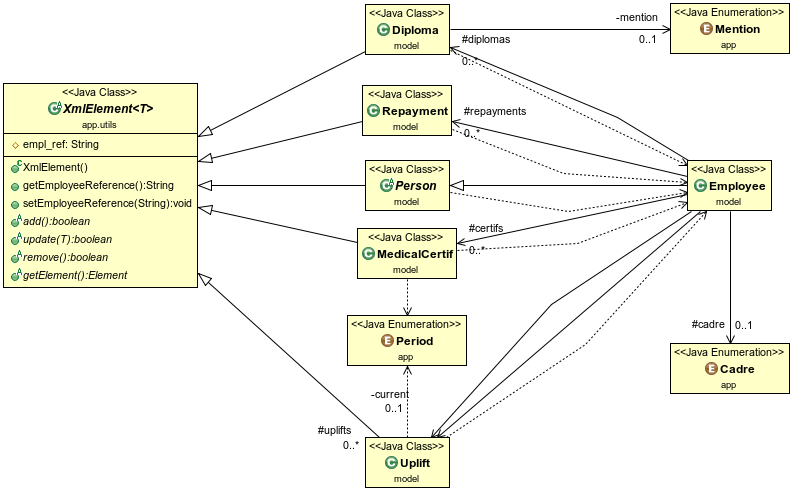
\includegraphics[width=11cm]{./diags/classes.png}
\end{center}
\end{frame}


\begin{frame}[fragile,label={sec:orgf76f778}]{Héritage de la classe \texttt{XmlElement}}
 \begin{quote}
La méthode \texttt{update()} prend un variable de type \texttt{T},\pause ce type est décrit avec un héritage de la classe \texttt{XmlElement} \pause
\end{quote}

\begin{minted}[linenos,firstnumber=1]{java}
public class Diploma extends XmlElement<Diploma> {
    /* les attributs du classe */
    @Override
    public boolean update(Diploma updated) {
        try {
            /* process la mise à jour */
            return true;
        } catch (Exception e) {
            System.err.println(e.getMessage());
            return false;
        }
    }
}
\end{minted}
\end{frame}
\section{L’Interface Graphique}
\label{sec:org877219e}
\begin{frame}[label={sec:org9d855c3}]{L’Interface Graphique}
\begin{center}
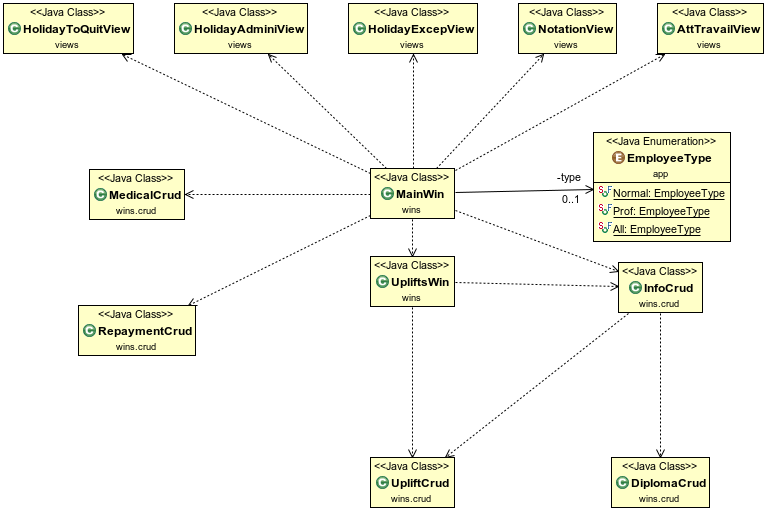
\includegraphics[width=10cm]{./diags/OverviewOnWinsAnd.png}
\end{center}
\end{frame}

\begin{frame}[fragile,label={sec:org597e26f}]{La fenêtre principale \texttt{MainWin}}
 \begin{center}
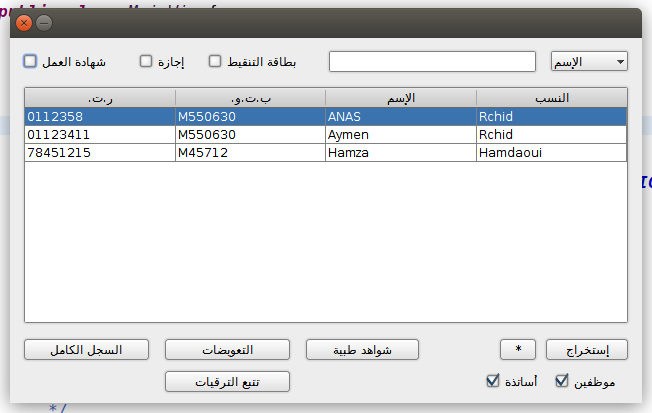
\includegraphics[width=10cm]{./diags/MainWin.png}
\end{center}
\end{frame}
\begin{frame}[fragile,label={sec:org494951d}]{La fenêtre de suivi des avancements de grade \texttt{UpliftsWin}}
 \begin{center}
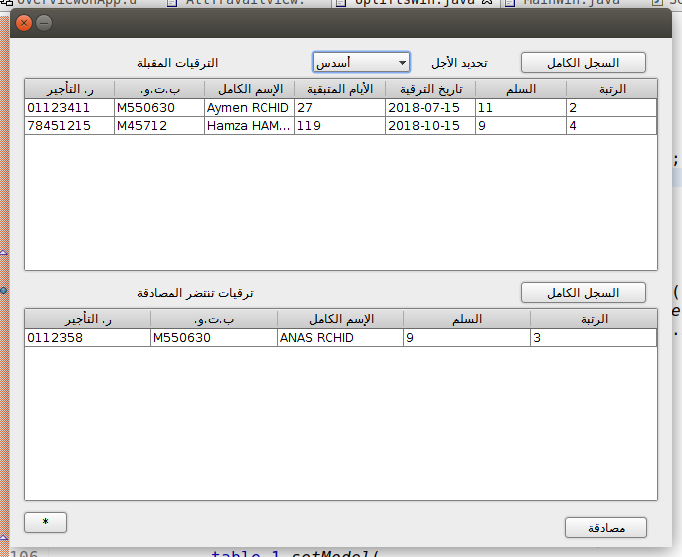
\includegraphics[width=9cm]{./diags/UpliftsWin.png}
\end{center}
\end{frame}

\begin{frame}[fragile,label={sec:org0ba1b6c}]{Gestion des Employés \texttt{InfoCrud}}
 \begin{center}
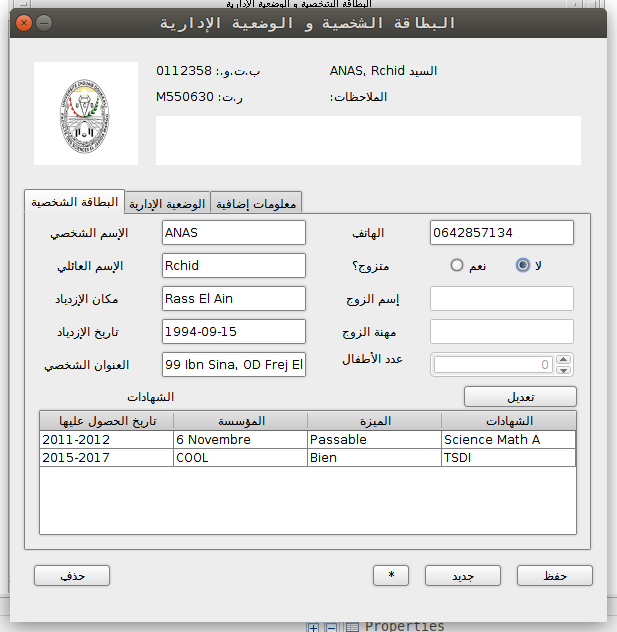
\includegraphics[width=7cm]{./diags/InfoWin.png}
\end{center}
\end{frame}

\begin{frame}[label={sec:org4374f8d}]{Démonstration}
\end{frame}

\section{Conclusion}
\label{sec:orga329362}
\begin{frame}[fragile,label={sec:org6c024d4}]{Conclusion}
 \begin{quote}
\emph{Ce projet a été sous plusieurs aspects riches d'enseignements.}
\emph{Le projet consistait à realiser une application permetant la gestion des carriers des ressoures humaines. C'etait une opportunité pour améliorer mes connaissances au matiere de codage \texttt{Java}.}\\

\emph{En conclusion, mon projet ma permetais de mettre en oeuvre mes competances scolaires, professionnelles et humaines pour un sujet intéresant. J'ai acquis des nouvelles compétances dans le domain de développement}
\end{quote}
\end{frame}

\begin{frame}[label={sec:org74a9c6a}]{Conclusion}
\begin{quote}
\emph{Merci de votre attention}
\end{quote}
\end{frame}
\end{document}